
% \subsection{Bench-marking CPU Utilization for UDP Affine Traffic}
% In this paper, we have focussed on server-type multi-tier applications
% which employ TCP communication across tiers. Our benchmarking experiments
% also spawned processes that opened TCP sockets and performed connection
% oriented communication. Here, we perform a brief experiment to observe
% the difference in CPU usage when UDP connectionless traffic is present 
% instead of TCP. Intuitively, the CPU usage would be higher due to the
% necessity of having to set up UDP socket for every datagram being sent
% across. In our custom UDP application, we use the same segment sizes
% as before, ranging from 1KB to 70KB and Fig.~\ref{udprx} presents the
% CPU utilization incurred at the receiving DomU in dispersed and
% colocated scenarios, respectively.


\subsection{Benchmarking of 1 Gbps link network usage}
\label{ref:1gbps}
In our experiments, we used network links with capacity 100 Mbps 
for network traffic
and found that CPU usage had a linear correlation with network usage.
This was the basis for using a linear regression modeling technique
for CPU estimation. However, in order for our approach to be valid
for 1 Gbps links, this linear correlation should hold in a setup with
traffic up to 1 Gbps as well. To this end, we performed a benchmarking
exercise as before (with Xen), but with a 1 Gbps link, to answer
the following questions:
%We perform this study for the Xen virtualization environment here.
%The motivations of this study are two-fold:-
(i) Does the linear correlation of CPU to network usage still hold 
with 1 Gbps links?
(ii) Does using different capacity links between communicating VMs 
result in different CPU utilization at the VMs (and Dom0 for Xen)?

\begin{figure}[t]
\centering
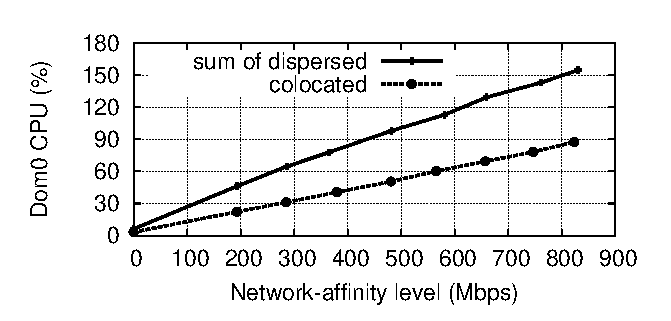
\includegraphics[scale=0.75]{jss-figures/new-aff-1G-benchmark/multi-bytetcp-1Gbps-nogsotsoboth-0iptabs-5120-dom0-cpu-vs-affine-curve.eps}
\caption{Dom0 Utilization over a 1Gbps link}
\label{fig:link1gbps}
\end{figure}



Fig.~\ref{fig:link1gbps} shows CPU utilization at Dom0
for network-affinity levels ranging from 100 to 900 Mbps, in 
both dispersed and colocated scenarios for segment size of
5KB. As can be seen, the CPU utilization is linearly correlated with
network rate in both the cases. 
% We made similar observations at the transmitting DomU as well. 
However, the magnitudes of CPU utilization
incurred for network rates $\le$ 100 Mbps over a 1 Gbps link are not the 
same as those observed during benchmarking with 100 Mbps links. 
%More
%specifically, CPU required to transmit or receive 50Mbps traffic 
%over a 100Mbps link is not the same as that required over a 1Gbps link.
This implies that network link bandwidth is an important
determinant of CPU utilization incurred at the transmitter and
receiver. So, if the cloud deployment has networks links or switches 
of heterogeneous capacities,
different CPU estimation models would need to be
developed for each link type.
Overall, we conclude that 
linear regression modeling approach can be applied for affinity-aware
CPU estimation even in deployments with 1 Gbps links. 

\subsection{Effect of colocation for data-centric applications}
The work in this paper is targeted towards multi-tiered service-oriented
applications such that the user issues a request and waits 
for a certain time (think-time) before firing the next request.
In such a scenario, where think-time intervals are relatively large
(as compared to response transmission time),
requests are issued at long enough intervals
such that observed network-affinity levels
in colocated and dispersed scenarios are the same. 
However, for data-centric applications 
where tiers exchange large amounts of data, the transmission
durations are significant and hence 
observed network-affinity levels in colocated
and dispersed placements are not same (for observation intervals
smaller than data transmission durations).
%Hence, performance of
%such applications would experience significant difference
%in colocated and dispersed scenarios. 
%For example, an 18 minute
%run of RUBiS workload would finish in 18 minutes in both 
%dispersed and colocated scenario. 
For example, with an application
that sends bulk data in an as-soon-as-possible manner, 
completion times may be sooner or later depending
on whether participating VMs are colocated or dispersed
and hence the network bandwidth available in each scenario. 
An enhanced model that estimates network-affinity level 
and resulting CPU utilization based on placement scenarios would
be required.
%This 
%implies that 
%change in relative placement for VMs of a data-centric application
%would result in change in affine network traffic rates as well,
%and CPU utilization on the target would be a function
%of the network rate in the new placement scenario. Thus, an
%extra step of predicting the resultant affine network rate
%is also needed in this case.

\subsection{Capacity planning for virtualized services}
An important aspect of migration of services from physical to virtual
environments (P2V) is estimation of resources needed to meet SLA
requirements
\cite{migrating-n-tier-apps, migrating-service-oriented, 
legacy-app-migration}.
%A capacity planning exercise is needed the estimation of total 
%resources needed
%to migrate a set of applications from physical to virtual (P2V transition)
As shown in our work, colocation
and dispersion of communicating tiers of an application can
result in differing CPU utilization for both DomUs and Dom0.
Thus, estimating CPU usage of two tiers individually
for the P2V transition will neglect the effects of affinity 
on their CPU usage.

Resource requirement in virtualized
environment depends on type of application being migrated
from physical to virtual. 
In \cite{profiling-and-modeling}, linear regression models
have been built to estimate virtual CPU usage from given
physical resource usage profiles. However, this has been 
done only for one tier (web server tier) of the application
and not for the other (database tier). Thus, it 
does not
consider both cases\textemdash{}colocation and dispersion\textemdash{}of 
location of the two tiers, and instead addresses only the
dispersed placement by default. In our work, we have demonstrated that 
virtualized CPU usage of both communicating tiers are
dependent on their relative placement also. Thus, during
the P2V transition, virtual CPU usage estimation should
also consider whether or not the communicating VMs are intended
to be colocated. Our idea is that for every VM that has
network communication with any other VM, the P2V CPU estimation
models presented in \cite{profiling-and-modeling} can be
used to predict its dispersed virtual CPU usage, and then
our \textit{colocation} model can be applied to this estimation
to predict the final virtual CPU usage. 


% Note that, this
% transitive approach to P2V CPU usage prediction closely
% couples the VM's CPU usage and its placement.

% In \cite{migrating-n-tier-apps},
% change in performance upon migration of n-tier applications 
% to different clouds is addressed and the causes identified, 
% whereas \cite{migrating-service-oriented, legacy-app-migration} focus
% on the processes, methods and tools needed for this P2V transition.
